\documentclass[aspectratio=169,11pt]{beamer}
% =====================================================================
%  pds-beamer.tex — Estilo común de las transparencias.
%
%  Uso (desde teoría/Tx/transparencias/):
%     \documentclass[aspectratio=169,11pt]{beamer}
%     % =====================================================================
%  pds-beamer.tex — Estilo común de las transparencias.
%
%  Uso (desde teoría/Tx/transparencias/):
%     \documentclass[aspectratio=169,11pt]{beamer}
%     % =====================================================================
%  pds-beamer.tex — Estilo común de las transparencias.
%
%  Uso (desde teoría/Tx/transparencias/):
%     \documentclass[aspectratio=169,11pt]{beamer}
%     \input{../../comun/pds-beamer}
%     \title{...}  \subtitle{Tema x · ...}
%     \begin{document}
%       \portada
%       ...
%     \end{document}
%  Compilar con:  latexmk -xelatex  (o «make» desde teoría/)
% =====================================================================

\usetheme{Boadilla}
\usecolortheme{orchid}
\usefonttheme{professionalfonts}
\setbeamercovered{transparent}
\setbeamersize{text margin left=0.8cm, text margin right=0.8cm}
\setbeamertemplate{navigation symbols}{}
\setbeamertemplate{itemize item}[square]
\setbeamertemplate{itemize subitem}[circle]
\setbeamertemplate{itemize subsubitem}[triangle]
\setbeamertemplate{enumerate item}[square]
\setbeamertemplate{enumerate subitem}[circle]
\setbeamertemplate{caption}{\raggedright\insertcaption\par}

\input{../../comun/pds-comun.tex}

% Tipografía: Fira Sans + Fira Math (legibles en proyector)
\usepackage{fontspec}
\usepackage{unicode-math}
% Se cargan por nombre de fichero para que funcionen con cualquier
% instalación de TeX Live (o MiKTeX) sin instalar fuentes en el sistema.
\setmainfont{FiraSans}[Extension=.otf, UprightFont=*-Regular, BoldFont=*-SemiBold,
  ItalicFont=*-Italic, BoldItalicFont=*-SemiBoldItalic]
\setsansfont{FiraSans}[Extension=.otf, UprightFont=*-Regular, BoldFont=*-SemiBold,
  ItalicFont=*-Italic, BoldItalicFont=*-SemiBoldItalic]
\setmonofont{FiraMono}[Extension=.otf, UprightFont=*-Regular, BoldFont=*-Medium, AutoFakeSlant=0.15, Scale=0.92]
\setmathfont{FiraMath-Regular.otf}
\setmathfont{latinmodern-math.otf}[range={"229B,"22EE,"22F1}]

% Colores del tema ajustados a la paleta común (más contraste)
\setbeamercolor{structure}{fg=pdsazul}
\setbeamercolor{alerted text}{fg=pdsrojo}
\setbeamercolor{example text}{fg=pdsverde}
\setbeamercolor{block title}{bg=pdsazul, fg=white}
\setbeamercolor{block body}{bg=pdsfondo}
\setbeamercolor{block title alerted}{bg=pdsrojo, fg=white}
\setbeamercolor{block body alerted}{bg=pdsrojo!6}
\setbeamercolor{block title example}{bg=pdsverde, fg=white}
\setbeamercolor{block body example}{bg=pdsverde!6}
\setbeamercolor{frametitle}{fg=pdsazul, bg=white}
\setbeamerfont{frametitle}{size=\large, series=\bfseries}
\setbeamerfont{block title}{size=\normalsize, series=\bfseries}
\setbeamertemplate{blocks}[rounded][shadow=false]

% Logo en la esquina superior derecha de cada transparencia
\pgfdeclareimage[height=0.8cm]{logo}{../../comun/ucm.png}
\addtobeamertemplate{frametitle}{}{%
  \begin{tikzpicture}[remember picture, overlay]
    \node[anchor=north east, inner sep=0pt] at ([xshift=-0.25cm, yshift=-0.2cm]current page.north east) {\pgfuseimage{logo}};
  \end{tikzpicture}}

% Datos de portada
\author[\autorescorto]{\autores}
\institute[UCM]{\footnotesize\departamento\\\universidad}
\date[\curso]{\footnotesize\grado\\\curso}

\newcommand{\portada}{%
  \begin{frame}[plain]
    \begin{center}
      
\includegraphics[height=1.9cm]{../../comun/ucm.png}
    \end{center}
    \vspace{-0.4cm}
    \titlepage
  \end{frame}}

% Índice al empezar cada sección
\AtBeginSection[]{%
  \begin{frame}{Contenido}
    \tableofcontents[currentsection, hideothersubsections]
  \end{frame}}

\renewcommand{\pdscodesize}{\scriptsize}

% Utilidades
% \herramienta{T1-convolucion-continua}: enlace a la página publicada de
% herramientas/html (se abre en el navegador, sin instalar nada).
% \herramientaservidor{server/....py}: app que necesita Python (bokeh serve).
\newcommand{\urlherramientas}{https://ucm-237.github.io/PdS/}
\newcommand{\herramienta}[1]{%
  \par\vfill\hfill{\scriptsize\color{pdsgris}\faIcon\ \href{\urlherramientas#1.html}{Herramienta interactiva: \texttt{#1}}}}
\newcommand{\herramientaservidor}[1]{%
  \par\vfill\hfill{\scriptsize\color{pdsgris}\faIcon\ Herramienta interactiva (con Python): \texttt{herramientas/#1}}}
\newcommand{\faIcon}{\textbf{▶}}
\newcommand{\gris}[1]{{\color{pdsgris}#1}}
\newcommand{\nota}[1]{\par\vspace{2pt}{\footnotesize\color{pdsgris}\textit{#1}}\par}
% Nota sobre una errata de versiones anteriores (solo con \ERRATAS)
\newcommand{\errata}[1]{\iferratas\nota{Errata de versiones anteriores: #1}\fi}
\newcommand{\apuntes}[1]{\nota{Más detalle en los apuntes, #1.}}

% Bloques con nombre en castellano
\newenvironment{definicion}[1][Definición]{\begin{block}{#1}}{\end{block}}
\newenvironment{importante}[1][Importante]{\begin{alertblock}{#1}}{\end{alertblock}}
\newenvironment{ejemplo}[1][Ejemplo]{\begin{exampleblock}{#1}}{\end{exampleblock}}

%     \title{...}  \subtitle{Tema x · ...}
%     \begin{document}
%       \portada
%       ...
%     \end{document}
%  Compilar con:  latexmk -xelatex  (o «make» desde teoría/)
% =====================================================================

\usetheme{Boadilla}
\usecolortheme{orchid}
\usefonttheme{professionalfonts}
\setbeamercovered{transparent}
\setbeamersize{text margin left=0.8cm, text margin right=0.8cm}
\setbeamertemplate{navigation symbols}{}
\setbeamertemplate{itemize item}[square]
\setbeamertemplate{itemize subitem}[circle]
\setbeamertemplate{itemize subsubitem}[triangle]
\setbeamertemplate{enumerate item}[square]
\setbeamertemplate{enumerate subitem}[circle]
\setbeamertemplate{caption}{\raggedright\insertcaption\par}

% =====================================================================
%  pds-comun.tex — Paquetes, colores y estilos de código comunes a
%  transparencias, apuntes y hojas de ejercicios. Compilar con XeLaTeX.
%  No cargar directamente: lo cargan pds-beamer.tex y pds-apuntes.tex.
% =====================================================================

\usepackage{polyglossia}
\setmainlanguage{spanish}
\usepackage{mathtools}
\usepackage{graphicx}
\usepackage{booktabs}
\usepackage{multirow}
\usepackage{array}
\usepackage{xcolor}
\usepackage{tikz}
\usetikzlibrary{positioning,arrows.meta,calc,shapes.geometric,decorations.pathreplacing}
\usepackage{listings}
\usepackage{siunitx}
\sisetup{output-decimal-marker={,}, group-separator={\,}, per-mode=symbol}

% Notas de erratas de versiones anteriores: no se imprimen salvo que se
% defina \ERRATAS antes de cargar el estilo (make ERRATAS=1)
\newif\iferratas
\ifdefined\ERRATAS \erratastrue \fi

% Ruta común (logo y figuras compartidas)
\providecommand{\rutacomun}{../../comun/}
\input{\rutacomun datos.tex}

% ---------------------------------------------------------------------
%  Paleta (la misma que usan las figuras generadas con Python,
%  ver comun/pds_estilo.py)
% ---------------------------------------------------------------------
\definecolor{pdsazul}{HTML}{2B3A8C}
\definecolor{pdsrojo}{HTML}{C0392B}
\definecolor{pdsverde}{HTML}{1E7B4F}
\definecolor{pdsnaranja}{HTML}{D9822B}
\definecolor{pdsgris}{HTML}{5A5A66}
\definecolor{pdsfondo}{HTML}{F3F4FA}
\definecolor{pdscodigo}{HTML}{F7F7F2}

% ---------------------------------------------------------------------
%  Diagramas de bloques (TikZ)
% ---------------------------------------------------------------------
\tikzset{
  bloque/.style={rectangle, rounded corners=2pt, draw=pdsazul!80, fill=pdsfondo,
                 very thick, minimum height=8mm, minimum width=14mm, align=center},
  sumador/.style={circle, draw=pdsazul!80, fill=pdsfondo, thick, inner sep=1.5pt},
  flecha/.style={-{Stealth[length=2.2mm]}, thick, pdsgris},
}

% ---------------------------------------------------------------------
%  Código: Python y Matlab en paralelo
% ---------------------------------------------------------------------
\newcommand{\pdscodesize}{\footnotesize}
\lstdefinestyle{pds}{
  basicstyle=\ttfamily\pdscodesize,
  keywordstyle=\color{pdsazul}\bfseries,
  commentstyle=\color{pdsverde}\itshape,
  stringstyle=\color{pdsrojo},
  numbers=none,
  backgroundcolor=\color{pdscodigo},
  frame=single, rulecolor=\color{pdsgris!40}, framerule=0.4pt,
  xleftmargin=2pt, xrightmargin=2pt, aboveskip=2pt, belowskip=2pt,
  columns=fullflexible, keepspaces=true,
  showstringspaces=false, breaklines=true, tabsize=4,
  upquote=true,
  % Con XeLaTeX, listings desordena los caracteres no ASCII junto a
  % dígitos («2π» sale «π2»): se sustituyen por su versión matemática.
  literate={π}{{$\pi$}}1 {δ}{{$\delta$}}1 {ω}{{$\omega$}}1 {Ω}{{$\Omega$}}1
           {≈}{{$\approx$}}1 {µ}{{$\mu$}}1 {·}{{$\cdot$}}1 {α}{{$\alpha$}}1
           {á}{{á}}1 {é}{{é}}1 {í}{{í}}1 {ó}{{ó}}1 {ú}{{ú}}1 {ñ}{{ñ}}1 {¿}{{¿}}1,
}
\lstdefinestyle{python}{style=pds, language=Python,
  morekeywords={as,True,False,None}}
\lstdefinestyle{matlab}{style=pds, language=Matlab,
  morekeywords={function,end,true,false}}

% \codigo{<ruta sin extensión>} muestra el mismo ejemplo en Python
% y en Matlab, uno al lado del otro. Los ficheros viven en
% ../codigo/python/<nombre>.py y ../codigo/matlab/<nombre>.m y se
% ejecutan en las pruebas (make prueba-codigo).
\newcommand{\rutacodigo}{../codigo/}
\newcommand{\codigoetiqueta}[1]{{\sffamily\scriptsize\bfseries\color{pdsgris}#1}}
\newcommand{\codigo}[2][]{%
  \par\noindent
  \begin{minipage}[t]{0.495\linewidth}
    \codigoetiqueta{Python}\par\vspace{1pt}
    \lstinputlisting[style=python,#1]{\rutacodigo python/#2.py}
  \end{minipage}\hfill
  \begin{minipage}[t]{0.495\linewidth}
    \codigoetiqueta{Matlab}\par\vspace{1pt}
    \lstinputlisting[style=matlab,#1]{\rutacodigo matlab/#2.m}
  \end{minipage}\par}

\input{\rutacomun notacion.tex}


% Tipografía: Fira Sans + Fira Math (legibles en proyector)
\usepackage{fontspec}
\usepackage{unicode-math}
% Se cargan por nombre de fichero para que funcionen con cualquier
% instalación de TeX Live (o MiKTeX) sin instalar fuentes en el sistema.
\setmainfont{FiraSans}[Extension=.otf, UprightFont=*-Regular, BoldFont=*-SemiBold,
  ItalicFont=*-Italic, BoldItalicFont=*-SemiBoldItalic]
\setsansfont{FiraSans}[Extension=.otf, UprightFont=*-Regular, BoldFont=*-SemiBold,
  ItalicFont=*-Italic, BoldItalicFont=*-SemiBoldItalic]
\setmonofont{FiraMono}[Extension=.otf, UprightFont=*-Regular, BoldFont=*-Medium, AutoFakeSlant=0.15, Scale=0.92]
\setmathfont{FiraMath-Regular.otf}
\setmathfont{latinmodern-math.otf}[range={"229B,"22EE,"22F1}]

% Colores del tema ajustados a la paleta común (más contraste)
\setbeamercolor{structure}{fg=pdsazul}
\setbeamercolor{alerted text}{fg=pdsrojo}
\setbeamercolor{example text}{fg=pdsverde}
\setbeamercolor{block title}{bg=pdsazul, fg=white}
\setbeamercolor{block body}{bg=pdsfondo}
\setbeamercolor{block title alerted}{bg=pdsrojo, fg=white}
\setbeamercolor{block body alerted}{bg=pdsrojo!6}
\setbeamercolor{block title example}{bg=pdsverde, fg=white}
\setbeamercolor{block body example}{bg=pdsverde!6}
\setbeamercolor{frametitle}{fg=pdsazul, bg=white}
\setbeamerfont{frametitle}{size=\large, series=\bfseries}
\setbeamerfont{block title}{size=\normalsize, series=\bfseries}
\setbeamertemplate{blocks}[rounded][shadow=false]

% Logo en la esquina superior derecha de cada transparencia
\pgfdeclareimage[height=0.8cm]{logo}{../../comun/ucm.png}
\addtobeamertemplate{frametitle}{}{%
  \begin{tikzpicture}[remember picture, overlay]
    \node[anchor=north east, inner sep=0pt] at ([xshift=-0.25cm, yshift=-0.2cm]current page.north east) {\pgfuseimage{logo}};
  \end{tikzpicture}}

% Datos de portada
\author[\autorescorto]{\autores}
\institute[UCM]{\footnotesize\departamento\\\universidad}
\date[\curso]{\footnotesize\grado\\\curso}

\newcommand{\portada}{%
  \begin{frame}[plain]
    \begin{center}
      
\includegraphics[height=1.9cm]{../../comun/ucm.png}
    \end{center}
    \vspace{-0.4cm}
    \titlepage
  \end{frame}}

% Índice al empezar cada sección
\AtBeginSection[]{%
  \begin{frame}{Contenido}
    \tableofcontents[currentsection, hideothersubsections]
  \end{frame}}

\renewcommand{\pdscodesize}{\scriptsize}

% Utilidades
% \herramienta{T1-convolucion-continua}: enlace a la página publicada de
% herramientas/html (se abre en el navegador, sin instalar nada).
% \herramientaservidor{server/....py}: app que necesita Python (bokeh serve).
\newcommand{\urlherramientas}{https://ucm-237.github.io/PdS/}
\newcommand{\herramienta}[1]{%
  \par\vfill\hfill{\scriptsize\color{pdsgris}\faIcon\ \href{\urlherramientas#1.html}{Herramienta interactiva: \texttt{#1}}}}
\newcommand{\herramientaservidor}[1]{%
  \par\vfill\hfill{\scriptsize\color{pdsgris}\faIcon\ Herramienta interactiva (con Python): \texttt{herramientas/#1}}}
\newcommand{\faIcon}{\textbf{▶}}
\newcommand{\gris}[1]{{\color{pdsgris}#1}}
\newcommand{\nota}[1]{\par\vspace{2pt}{\footnotesize\color{pdsgris}\textit{#1}}\par}
% Nota sobre una errata de versiones anteriores (solo con \ERRATAS)
\newcommand{\errata}[1]{\iferratas\nota{Errata de versiones anteriores: #1}\fi}
\newcommand{\apuntes}[1]{\nota{Más detalle en los apuntes, #1.}}

% Bloques con nombre en castellano
\newenvironment{definicion}[1][Definición]{\begin{block}{#1}}{\end{block}}
\newenvironment{importante}[1][Importante]{\begin{alertblock}{#1}}{\end{alertblock}}
\newenvironment{ejemplo}[1][Ejemplo]{\begin{exampleblock}{#1}}{\end{exampleblock}}

%     \title{...}  \subtitle{Tema x · ...}
%     \begin{document}
%       \portada
%       ...
%     \end{document}
%  Compilar con:  latexmk -xelatex  (o «make» desde teoría/)
% =====================================================================

\usetheme{Boadilla}
\usecolortheme{orchid}
\usefonttheme{professionalfonts}
\setbeamercovered{transparent}
\setbeamersize{text margin left=0.8cm, text margin right=0.8cm}
\setbeamertemplate{navigation symbols}{}
\setbeamertemplate{itemize item}[square]
\setbeamertemplate{itemize subitem}[circle]
\setbeamertemplate{itemize subsubitem}[triangle]
\setbeamertemplate{enumerate item}[square]
\setbeamertemplate{enumerate subitem}[circle]
\setbeamertemplate{caption}{\raggedright\insertcaption\par}

% =====================================================================
%  pds-comun.tex — Paquetes, colores y estilos de código comunes a
%  transparencias, apuntes y hojas de ejercicios. Compilar con XeLaTeX.
%  No cargar directamente: lo cargan pds-beamer.tex y pds-apuntes.tex.
% =====================================================================

\usepackage{polyglossia}
\setmainlanguage{spanish}
\usepackage{mathtools}
\usepackage{graphicx}
\usepackage{booktabs}
\usepackage{multirow}
\usepackage{array}
\usepackage{xcolor}
\usepackage{tikz}
\usetikzlibrary{positioning,arrows.meta,calc,shapes.geometric,decorations.pathreplacing}
\usepackage{listings}
\usepackage{siunitx}
\sisetup{output-decimal-marker={,}, group-separator={\,}, per-mode=symbol}

% Notas de erratas de versiones anteriores: no se imprimen salvo que se
% defina \ERRATAS antes de cargar el estilo (make ERRATAS=1)
\newif\iferratas
\ifdefined\ERRATAS \erratastrue \fi

% Ruta común (logo y figuras compartidas)
\providecommand{\rutacomun}{../../comun/}
\input{\rutacomun datos.tex}

% ---------------------------------------------------------------------
%  Paleta (la misma que usan las figuras generadas con Python,
%  ver comun/pds_estilo.py)
% ---------------------------------------------------------------------
\definecolor{pdsazul}{HTML}{2B3A8C}
\definecolor{pdsrojo}{HTML}{C0392B}
\definecolor{pdsverde}{HTML}{1E7B4F}
\definecolor{pdsnaranja}{HTML}{D9822B}
\definecolor{pdsgris}{HTML}{5A5A66}
\definecolor{pdsfondo}{HTML}{F3F4FA}
\definecolor{pdscodigo}{HTML}{F7F7F2}

% ---------------------------------------------------------------------
%  Diagramas de bloques (TikZ)
% ---------------------------------------------------------------------
\tikzset{
  bloque/.style={rectangle, rounded corners=2pt, draw=pdsazul!80, fill=pdsfondo,
                 very thick, minimum height=8mm, minimum width=14mm, align=center},
  sumador/.style={circle, draw=pdsazul!80, fill=pdsfondo, thick, inner sep=1.5pt},
  flecha/.style={-{Stealth[length=2.2mm]}, thick, pdsgris},
}

% ---------------------------------------------------------------------
%  Código: Python y Matlab en paralelo
% ---------------------------------------------------------------------
\newcommand{\pdscodesize}{\footnotesize}
\lstdefinestyle{pds}{
  basicstyle=\ttfamily\pdscodesize,
  keywordstyle=\color{pdsazul}\bfseries,
  commentstyle=\color{pdsverde}\itshape,
  stringstyle=\color{pdsrojo},
  numbers=none,
  backgroundcolor=\color{pdscodigo},
  frame=single, rulecolor=\color{pdsgris!40}, framerule=0.4pt,
  xleftmargin=2pt, xrightmargin=2pt, aboveskip=2pt, belowskip=2pt,
  columns=fullflexible, keepspaces=true,
  showstringspaces=false, breaklines=true, tabsize=4,
  upquote=true,
  % Con XeLaTeX, listings desordena los caracteres no ASCII junto a
  % dígitos («2π» sale «π2»): se sustituyen por su versión matemática.
  literate={π}{{$\pi$}}1 {δ}{{$\delta$}}1 {ω}{{$\omega$}}1 {Ω}{{$\Omega$}}1
           {≈}{{$\approx$}}1 {µ}{{$\mu$}}1 {·}{{$\cdot$}}1 {α}{{$\alpha$}}1
           {á}{{á}}1 {é}{{é}}1 {í}{{í}}1 {ó}{{ó}}1 {ú}{{ú}}1 {ñ}{{ñ}}1 {¿}{{¿}}1,
}
\lstdefinestyle{python}{style=pds, language=Python,
  morekeywords={as,True,False,None}}
\lstdefinestyle{matlab}{style=pds, language=Matlab,
  morekeywords={function,end,true,false}}

% \codigo{<ruta sin extensión>} muestra el mismo ejemplo en Python
% y en Matlab, uno al lado del otro. Los ficheros viven en
% ../codigo/python/<nombre>.py y ../codigo/matlab/<nombre>.m y se
% ejecutan en las pruebas (make prueba-codigo).
\newcommand{\rutacodigo}{../codigo/}
\newcommand{\codigoetiqueta}[1]{{\sffamily\scriptsize\bfseries\color{pdsgris}#1}}
\newcommand{\codigo}[2][]{%
  \par\noindent
  \begin{minipage}[t]{0.495\linewidth}
    \codigoetiqueta{Python}\par\vspace{1pt}
    \lstinputlisting[style=python,#1]{\rutacodigo python/#2.py}
  \end{minipage}\hfill
  \begin{minipage}[t]{0.495\linewidth}
    \codigoetiqueta{Matlab}\par\vspace{1pt}
    \lstinputlisting[style=matlab,#1]{\rutacodigo matlab/#2.m}
  \end{minipage}\par}

\input{\rutacomun notacion.tex}


% Tipografía: Fira Sans + Fira Math (legibles en proyector)
\usepackage{fontspec}
\usepackage{unicode-math}
% Se cargan por nombre de fichero para que funcionen con cualquier
% instalación de TeX Live (o MiKTeX) sin instalar fuentes en el sistema.
\setmainfont{FiraSans}[Extension=.otf, UprightFont=*-Regular, BoldFont=*-SemiBold,
  ItalicFont=*-Italic, BoldItalicFont=*-SemiBoldItalic]
\setsansfont{FiraSans}[Extension=.otf, UprightFont=*-Regular, BoldFont=*-SemiBold,
  ItalicFont=*-Italic, BoldItalicFont=*-SemiBoldItalic]
\setmonofont{FiraMono}[Extension=.otf, UprightFont=*-Regular, BoldFont=*-Medium, AutoFakeSlant=0.15, Scale=0.92]
\setmathfont{FiraMath-Regular.otf}
\setmathfont{latinmodern-math.otf}[range={"229B,"22EE,"22F1}]

% Colores del tema ajustados a la paleta común (más contraste)
\setbeamercolor{structure}{fg=pdsazul}
\setbeamercolor{alerted text}{fg=pdsrojo}
\setbeamercolor{example text}{fg=pdsverde}
\setbeamercolor{block title}{bg=pdsazul, fg=white}
\setbeamercolor{block body}{bg=pdsfondo}
\setbeamercolor{block title alerted}{bg=pdsrojo, fg=white}
\setbeamercolor{block body alerted}{bg=pdsrojo!6}
\setbeamercolor{block title example}{bg=pdsverde, fg=white}
\setbeamercolor{block body example}{bg=pdsverde!6}
\setbeamercolor{frametitle}{fg=pdsazul, bg=white}
\setbeamerfont{frametitle}{size=\large, series=\bfseries}
\setbeamerfont{block title}{size=\normalsize, series=\bfseries}
\setbeamertemplate{blocks}[rounded][shadow=false]

% Logo en la esquina superior derecha de cada transparencia
\pgfdeclareimage[height=0.8cm]{logo}{../../comun/ucm.png}
\addtobeamertemplate{frametitle}{}{%
  \begin{tikzpicture}[remember picture, overlay]
    \node[anchor=north east, inner sep=0pt] at ([xshift=-0.25cm, yshift=-0.2cm]current page.north east) {\pgfuseimage{logo}};
  \end{tikzpicture}}

% Datos de portada
\author[\autorescorto]{\autores}
\institute[UCM]{\footnotesize\departamento\\\universidad}
\date[\curso]{\footnotesize\grado\\\curso}

\newcommand{\portada}{%
  \begin{frame}[plain]
    \begin{center}
      
\includegraphics[height=1.9cm]{../../comun/ucm.png}
    \end{center}
    \vspace{-0.4cm}
    \titlepage
  \end{frame}}

% Índice al empezar cada sección
\AtBeginSection[]{%
  \begin{frame}{Contenido}
    \tableofcontents[currentsection, hideothersubsections]
  \end{frame}}

\renewcommand{\pdscodesize}{\scriptsize}

% Utilidades
% \herramienta{T1-convolucion-continua}: enlace a la página publicada de
% herramientas/html (se abre en el navegador, sin instalar nada).
% \herramientaservidor{server/....py}: app que necesita Python (bokeh serve).
\newcommand{\urlherramientas}{https://ucm-237.github.io/PdS/}
\newcommand{\herramienta}[1]{%
  \par\vfill\hfill{\scriptsize\color{pdsgris}\faIcon\ \href{\urlherramientas#1.html}{Herramienta interactiva: \texttt{#1}}}}
\newcommand{\herramientaservidor}[1]{%
  \par\vfill\hfill{\scriptsize\color{pdsgris}\faIcon\ Herramienta interactiva (con Python): \texttt{herramientas/#1}}}
\newcommand{\faIcon}{\textbf{▶}}
\newcommand{\gris}[1]{{\color{pdsgris}#1}}
\newcommand{\nota}[1]{\par\vspace{2pt}{\footnotesize\color{pdsgris}\textit{#1}}\par}
% Nota sobre una errata de versiones anteriores (solo con \ERRATAS)
\newcommand{\errata}[1]{\iferratas\nota{Errata de versiones anteriores: #1}\fi}
\newcommand{\apuntes}[1]{\nota{Más detalle en los apuntes, #1.}}

% Bloques con nombre en castellano
\newenvironment{definicion}[1][Definición]{\begin{block}{#1}}{\end{block}}
\newenvironment{importante}[1][Importante]{\begin{alertblock}{#1}}{\end{alertblock}}
\newenvironment{ejemplo}[1][Ejemplo]{\begin{exampleblock}{#1}}{\end{exampleblock}}

\graphicspath{{../figuras/}}

\title[T2 · Cuantificación]{Muestreo y reconstrucción de señales}
\subtitle{Tema 2 · Parte 3: cuantificación y codificación}

\begin{document}
\portada

% =====================================================================
\section{Cuantificación}

\begin{frame}{De señal discreta a señal digital}
  \begin{center}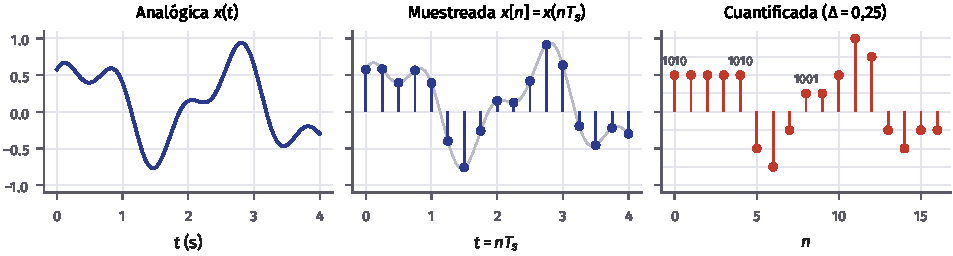
\includegraphics[width=0.85\linewidth]{muestreo_cuant_cod}\end{center}
  \begin{itemize}
    \item El muestreo discretiza el tiempo; la amplitud de $x[n]$ sigue siendo \alert{continua}.
    \item Un procesador solo almacena números con un número finito de bits.
    \item La \alert{cuantificación} asigna a cada muestra uno de $L$ valores permitidos:
    \[
      x_q[n]=Q\big[x[n]\big]
    \]
    \item La \alert{codificación} asigna a cada nivel una palabra binaria de $b$ bits.
  \end{itemize}
\end{frame}

\begin{frame}{Cuantificador uniforme}
  \begin{definicion}[Niveles y escalón de cuantificación]
    Con $b$ bits hay $L=2^b$ niveles separados por el \alert{escalón} (resolución) $\Delta$. Para una entrada en el margen $[-V,V)$, de fondo de escala $FS=2V$:
    \[
      \Delta=\frac{FS}{2^b}=\frac{2V}{2^b}
    \]
  \end{definicion}
  \begin{itemize}
    \item Es el convenio de los conversores A/D: $\Delta$ es el valor de \alert{1~LSB}.
    \item \gris{Otro convenio frecuente coloca el primer y el último nivel en los extremos del intervalo: $\Delta=\frac{x_{\max}-x_{\min}}{L-1}$. Las conclusiones son las mismas para $L$ grande.}
    \item Si $\abs{x}$ supera el margen, el cuantificador \alert{satura}: el error deja de estar acotado.
    \item Más bits $\Rightarrow$ menor $\Delta$ $\Rightarrow$ menor error, pero más memoria y un conversor más caro.
  \end{itemize}
\end{frame}

\begin{frame}{Redondeo y truncamiento}
  \begin{center}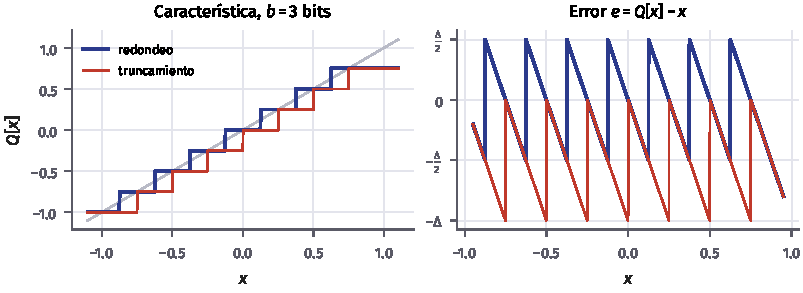
\includegraphics[height=0.4\textheight]{cuantificador}\end{center}
  \begin{columns}[T]
    \begin{column}{0.5\textwidth}
      \alert{Redondeo}: el nivel más cercano.
      \[
        Q[x]=\Delta\,\operatorname{round}\!\Big(\frac{x}{\Delta}\Big),\quad -\frac{\Delta}{2}\le e<\frac{\Delta}{2}
      \]
    \end{column}
    \begin{column}{0.5\textwidth}
      \alert{Truncamiento}: el nivel inmediatamente inferior.
      \[
        Q[x]=\Delta\,\Big\lfloor\frac{x}{\Delta}\Big\rfloor,\quad -\Delta<e\le 0
      \]
    \end{column}
  \end{columns}
  \medskip
  El \alert{error de cuantificación} es $e[n]=x_q[n]-x[n]$. La pérdida de información es irreversible: muchos valores van a parar al mismo nivel.
\end{frame}

\begin{frame}{Ejemplo: cuantificar $x[n]=0{,}9^n$}
  \begin{columns}[c]
    \begin{column}{0.45\textwidth}
      \small
      \begin{itemize}
        \item Para representar \alert{exactamente} $n=0,\dots,9$ hace falta $\Delta=10^{-9}$: $0{,}9^9=0{,}387420489$ tiene nueve decimales.
        \item Con un decimal, $\Delta=0{,}1$:
        \begin{itemize}\small
          \item truncando, $-0{,}1<e\le0$;
          \item redondeando, $\abs{e}\le0{,}05$.
        \end{itemize}
        \item El redondeo tiene media nula; el truncamiento introduce un sesgo de $-\Delta/2$.
      \end{itemize}
    \end{column}
    \begin{column}{0.53\textwidth}
      \footnotesize
      \renewcommand{\arraystretch}{1.15}
      \begin{tabular}{@{}rlllll@{}}
        \toprule
        & & \multicolumn{2}{c}{$x_q[n]$} & \multicolumn{2}{c}{$e[n]$}\\\cmidrule(lr){3-4}\cmidrule(l){5-6}
        $n$ & $x[n]$ & trunc. & red. & trunc. & red.\\\midrule
        0 & 1 & 1,0 & 1,0 & 0 & 0\\
        1 & 0,9 & 0,9 & 0,9 & 0 & 0\\
        2 & 0,81 & 0,8 & 0,8 & $-0{,}01$ & $-0{,}01$\\
        3 & 0,729 & 0,7 & 0,7 & $-0{,}029$ & $-0{,}029$\\
        4 & 0,6561 & 0,6 & 0,7 & $-0{,}0561$ & $0{,}0439$\\
        5 & 0,59049 & 0,5 & 0,6 & $-0{,}0905$ & $0{,}0095$\\
        6 & 0,53144 & 0,5 & 0,5 & $-0{,}0314$ & $-0{,}0314$\\
        7 & 0,47830 & 0,4 & 0,5 & $-0{,}0783$ & $0{,}0217$\\
        8 & 0,43047 & 0,4 & 0,4 & $-0{,}0305$ & $-0{,}0305$\\
        9 & 0,38742 & 0,3 & 0,4 & $-0{,}0874$ & $0{,}0126$\\\bottomrule
      \end{tabular}
    \end{column}
  \end{columns}
\end{frame}

% =====================================================================
\section{Ruido de cuantificación}

\begin{frame}{Modelo estadístico del error}
  \begin{columns}[c]
    \begin{column}{0.5\textwidth}
      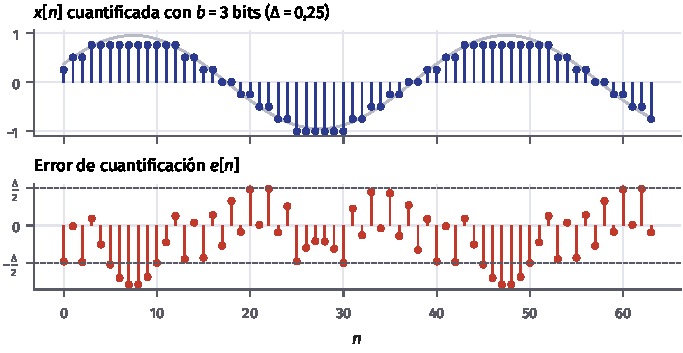
\includegraphics[width=\linewidth]{error_cuantificacion}
    \end{column}
    \begin{column}{0.48\textwidth}
      \small
      Si la señal cruza muchos niveles y no satura, el error es un \alert{ruido aditivo}, $x_q[n]=x[n]+e[n]$:
      \begin{itemize}\small
        \item $e[n]$ uniforme en $[-\Delta/2,\Delta/2)$ (redondeo).
        \item Incorrelado con $x[n]$, blanco y de media nula.
      \end{itemize}
      \begin{importante}
        \[
          \sigma_e^2=\frac{1}{\Delta}\int_{-\Delta/2}^{\Delta/2}e^2\dd e=\frac{\Delta^2}{12}
        \]
      \end{importante}
    \end{column}
  \end{columns}
  {\footnotesize\gris{El modelo falla si la señal es lenta o pequeña frente a $\Delta$. Las señales aleatorias se estudian en el Tema~6.}}
\end{frame}

\begin{frame}{Relación señal a ruido de cuantificación (SQNR)}
  \begin{columns}[c]
    \begin{column}{0.52\textwidth}
      \[
        \mathrm{SQNR}=10\log_{10}\frac{P_x}{\sigma_e^2}\ \text{dB}
      \]
      Para una sinusoide de amplitud $V$ (fondo de escala):
      \[
        P_x=\frac{V^2}{2},\qquad \sigma_e^2=\frac{\Delta^2}{12}=\frac{(2V)^2}{12\cdot2^{2b}}
      \]
      \begin{importante}
        \[
          \mathrm{SQNR}=10\log_{10}\Big(\frac32\,2^{2b}\Big)\approx 6{,}02\,b+1{,}76\ \text{dB}
        \]
      \end{importante}
    \end{column}
    \begin{column}{0.46\textwidth}
      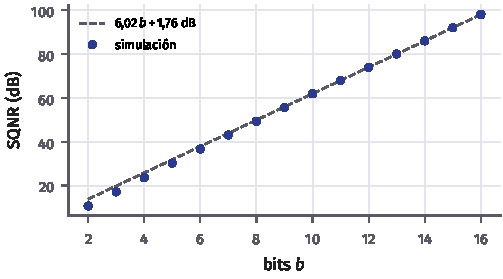
\includegraphics[width=\linewidth]{sqnr_bits}
      \begin{itemize}\small
        \item \alert{Cada bit añade unos 6\,dB}. CD (16 bits): unos 98\,dB.
        \item Con amplitud $V/10$ se pierden 20\,dB.
      \end{itemize}
    \end{column}
  \end{columns}
  \herramienta{T2-cuantificacion}
\end{frame}

\begin{frame}{En código: SQNR de un cuantificador}
  \codigo{cuantificacion}
  \nota{Con $b=8$ se mide $\mathrm{SQNR}\approx49{,}7$\,dB, frente a los $49{,}9$\,dB del modelo (la amplitud es $0{,}99\,V$).}
\end{frame}

% =====================================================================
\section{Codificación y conversores}

\begin{frame}{Codificación}
  \begin{columns}[c]
    \begin{column}{0.55\textwidth}
      \begin{itemize}
        \item $b$ bits representan $2^b$ palabras distintas; para $L$ niveles:
        \[
          2^b\ge L\quad\Longrightarrow\quad b\ge\log_2L
        \]
        \item \alert{Ejemplo}: $L=6$ niveles, $\log_26\approx2{,}585$, luego $b=3$ bits.
        \item Códigos habituales para un margen bipolar:
        \begin{itemize}\small
          \item \alert{binario desplazado}: $k+2^{b-1}$;
          \item \alert{complemento a dos}: el de la aritmética de los procesadores.
        \end{itemize}
      \end{itemize}
    \end{column}
    \begin{column}{0.42\textwidth}
      \footnotesize
      \renewcommand{\arraystretch}{1.1}
      \begin{tabular}{@{}rrcc@{}}
        \toprule
        $k$ & $x_q=k\Delta$ & desplazado & C2\\\midrule
        3 & $3\Delta$ & 111 & 011\\
        2 & $2\Delta$ & 110 & 010\\
        1 & $\Delta$ & 101 & 001\\
        0 & 0 & 100 & 000\\
        $-1$ & $-\Delta$ & 011 & 111\\
        $-2$ & $-2\Delta$ & 010 & 110\\
        $-3$ & $-3\Delta$ & 001 & 101\\
        $-4$ & $-4\Delta$ & 000 & 100\\\bottomrule
      \end{tabular}

      \gris{$b=3$, margen $[-4\Delta,4\Delta)$.}
    \end{column}
  \end{columns}
\end{frame}

\begin{frame}{Parámetros de un conversor A/D}
  \begin{itemize}
    \item \alert{Resolución} $b$ y \alert{tensión de referencia} $V_{\text{ref}}$. Margen unipolar $[0,V_{\text{ref}})$:
    \[
      1\,\text{LSB}=\Delta=\frac{V_{\text{ref}}}{2^b}
    \]
    \item \alert{Rango dinámico}: cociente entre la mayor y la menor amplitud distinguibles,
    \[
      \mathrm{DR}=20\log_{10}\frac{V_{\text{ref}}}{\Delta}=20\log_{10}2^b\approx6{,}02\,b\ \text{dB}
    \]
    \item \alert{Frecuencia de muestreo} máxima y tiempo de conversión.
    \item Arquitecturas: flash (rápida, pocos bits), aproximaciones sucesivas (SAR), sigma-delta (muchos bits, sobremuestreo; parte~4).
  \end{itemize}
  \begin{ejemplo}[Microcontrolador con A/D de 10 bits y $V_{\text{ref}}=3{,}3$\,V]
    $\Delta=3{,}3/1024\approx3{,}22$\,mV, $\mathrm{DR}\approx60{,}2$\,dB y, para una sinusoide a fondo de escala, $\mathrm{SQNR}\approx62$\,dB.
  \end{ejemplo}
\end{frame}

% =====================================================================
\section*{Resumen}
\begin{frame}{Conceptos importantes}
  \begin{columns}[T]
    \begin{column}{0.5\textwidth}
      \begin{itemize}
        \item Cuantificar es aproximar la amplitud: $x_q[n]=Q[x[n]]$.
        \item $L=2^b$ niveles, $\Delta=FS/2^b$.
        \item Redondeo: $\abs{e}\le\Delta/2$; truncamiento: $-\Delta<e\le0$.
        \item Modelo de ruido: $e[n]$ uniforme, $\sigma_e^2=\Delta^2/12$.
      \end{itemize}
    \end{column}
    \begin{column}{0.5\textwidth}
      \begin{itemize}
        \item $\mathrm{SQNR}\approx6{,}02\,b+1{,}76$\,dB a fondo de escala.
        \item Codificar $L$ niveles: $b\ge\log_2L$.
        \item Conversor A/D: $\Delta=V_{\text{ref}}/2^b$, $\mathrm{DR}\approx6{,}02\,b$\,dB.
      \end{itemize}
    \end{column}
  \end{columns}
  \bigskip
  \gris{Apuntes del Tema 2, sección 5 · Hoja de ejercicios, ejercicios 11–13.}
\end{frame}

\end{document}
